\section{COLORMAP Image Colormap Function}

\subsection{Usage}

Changes the colormap for the current figure.  The generic syntax 
for its use is
\begin{verbatim}
  colormap(map)
\end{verbatim}
where \verb|map| is a an array organized as \verb|3 \times N|),
which defines the RGB (Red Green Blue) coordinates for each color in the
colormap.  You can also use the function with no arguments to recover
the current colormap
\begin{verbatim}
  map = colormap
\end{verbatim}
\subsection{Function Internals}

Assuming that the contents of the colormap function argument \verb|c| are 
labeled as:
\[
  c = \begin{bmatrix}
    r_1 & g_1 & b_1 \\
    r_1 & g_2 & b_2 \\
    r_1 & g_3 & b_3 \\
    \vdots & \vdots & \vdots 
      \end{bmatrix} 
\]
then these columns for the RGB coordinates of pixel in the mapped image.
Assume that the image occupies the range $[a,b]$.  Then the RGB color 
of each pixel depends on the value $x$ via the following integer
\[
  k = 1 + \lfloor 256 \frac{x-a}{b-a} \rfloor,
\]
so that a pixel corresponding to image value $x$ will receive RGB color 
$[r_k,g_k,b_k]$.
Colormaps are generally used to pseudo color images to enhance 
visibility of features, etc.
\subsection{Examples}

We start by creating a smoothly varying image of a 2D Gaussian pulse.
\begin{verbatim}
--> x = linspace(-1,1,512)'*ones(1,512);
--> y = x';
--> Z = exp(-(x.^2+y.^2)/0.3);
--> image(Z);
\end{verbatim}
which we display with the default (grayscale) colormap here.


\centerline{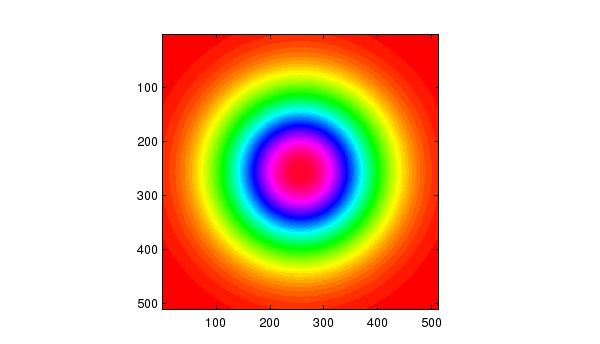
\includegraphics[width=8cm]{colormap1}}


Next we switch to the \verb|copper| colormap, and redisplay the image.
\begin{verbatim}
--> colormap(copper);
--> image(Z);
\end{verbatim}
which results in the following image.


\centerline{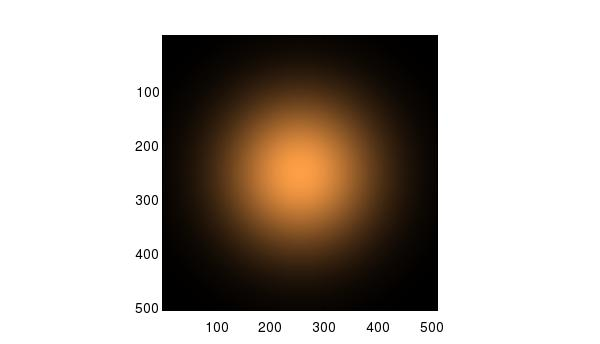
\includegraphics[width=8cm]{colormap2}}


If we capture the output of the \verb|copper| command and plot it, we obtain
the following result:
\begin{verbatim}
--> a = copper;
--> plot(a);
\end{verbatim}


\centerline{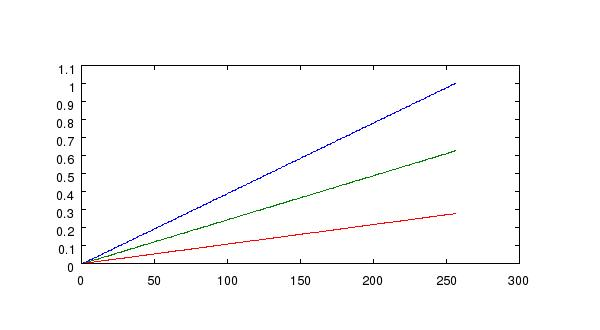
\includegraphics[width=8cm]{colormap3}}


Note that in the output that each of the color components are linear functions
of the index, with the ratio between the red, blue and green components remaining
constant as a function of index.  The result is an intensity map with a copper
tint.  We can similarly construct a colormap of our own by defining the 
three components seperately.  For example, suppose we take three gaussian
curves, one for each color, centered on different parts of the index space:
\begin{verbatim}
--> t = linspace(0,1,256);
--> A = [exp(-(t-1.0).^2/0.1);exp(-(t-0.5).^2/0.1);exp(-t.^2/0.1)]';
--> plot(A);
\end{verbatim}


\centerline{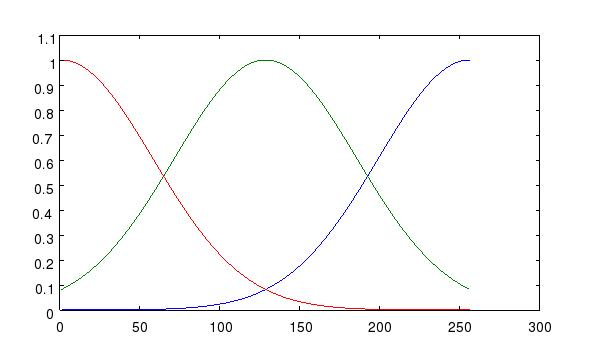
\includegraphics[width=8cm]{colormap4}}


The resulting image has dark bands in it near the color transitions.
\begin{verbatim}
--> image(Z);
--> colormap(A);
\end{verbatim}


\centerline{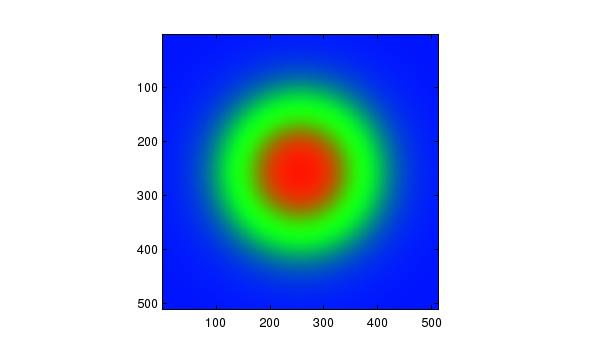
\includegraphics[width=8cm]{colormap5}}


These dark bands are a result of the nonuniform color intensity, which 
we can correct for by renormalizing each color to have the same norm.
\begin{verbatim}
--> w = sqrt(sum(A'.^2));
--> sA = diag(1./w)*A;
--> plot(A);
\end{verbatim}


\centerline{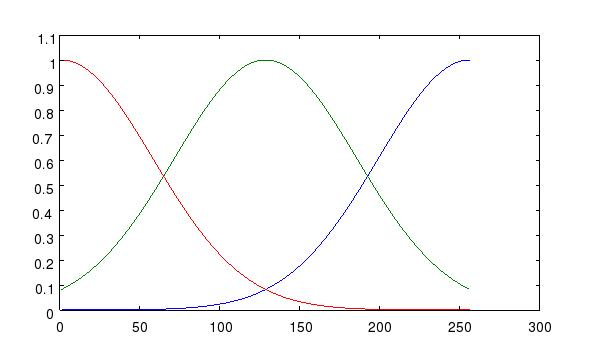
\includegraphics[width=8cm]{colormap6}}


The resulting image has no more dark bands.
\begin{verbatim}
--> image(Z);
--> colormap(A);
\end{verbatim}


\centerline{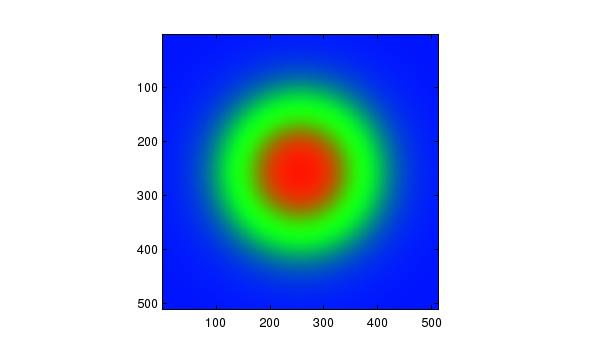
\includegraphics[width=8cm]{colormap7}}

